\section{Diagramme}

\subsection{Objektdiagramm (\textit{object diagram})\balzert{21}}
	\begin{multicols}{2}
		Momentaufnahme / Schnappschuss des Systems. \\
		Beschreibt Objekte, Attributwerte, Objektbeziehungen zu einem bestimmten Zeitpunkt. \\
	\columnbreak
		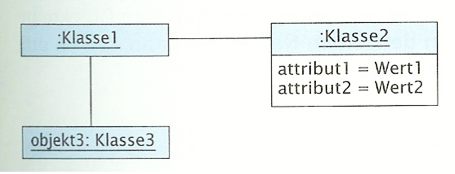
\includegraphics[width=5cm]{./images/objektdiagramm.png}
	\end{multicols}

\subsection{Use-Case Diagramm}
	Ein Use-Case spezifiziert eine Sequenz von Aktionen
	\begin{description}
		\item[Akteur] ist eine Rolle, die ein Benutzer des Systems spielt. Jeder
		Akteur hat einen Einfluss uaf das System. Befindet sich stets ausserhalb des Systems\\
	\end{description}